% !TEX program = xelatex

\documentclass{resume}
\usepackage{graphicx}
\usepackage{tabu}
\usepackage{multirow}
%\usepackage{zh_CN-Adobefonts_external} % Simplified Chinese Support using external fonts (./fonts/zh_CN-Adobe/)
%\usepackage{zh_CN-Adobefonts_internal} % Simplified Chinese Support using system fonts

\begin{document}
\pagenumbering{gobble} % suppress displaying page number

\large{
  \begin{tabu}{ c l }
   \multirow{5}{1in}{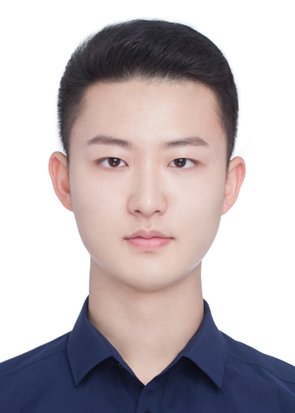
\includegraphics[width=0.88in]{avatar-1}} & \\ & \scshape \LARGE {\, Sun Dongxu}  \\
    & \quad \email{371211947@qq.com}  \\
    & \quad \phone{(+86) 189-7308-9012}  \\
    & \quad \github{https://github.com/sundongxu} \\
    & \quad 
\includegraphics[scale=0.02]{blog.pdf}{\ http://dongdongdong.me}
  \end{tabu} 
  \\ \\ 

\section{\faGraduationCap\ Education}
\datedsubsection{\textbf{Nanjing University (NJU)}, Jiangsu, China}{2016 -- Present}
\textit{Master student} in Computer Science (CS)
\datedsubsection{\textbf{Dalian University of Technology (DUT)}, Liaoning, China}{2012 -- 2016}
\textit{B.S.} in Software Engineering (SE)

\section{\faUsers\ Experience}
\datedsubsection{\textbf{Tencent Inc.} Shenzhen, China}{2015.08 -- 2016.02}
\role{Intern}{Mobile Developer}
\begin{itemize}
  \item Implemented features in Yingyongbao including native navigation revision, NPC pop-up window, new version of smart card, icon inside the games, which had already been tested and published
  \item Won the 2nd and the 3rd prizes in the basketball competitions on behalf of Yingyongbao and MIG, respectively 
\end{itemize}

\datedsubsection{\textbf{RDMA Network Middlebox}}{2017.03 -- 2017.10}
\role{C++/C}{Research Project, collaborated with classmates}
\begin{itemize}
  \item Support the upper applications to replace native TCP/IP protocol stack with RDMA (Message/Memory Semantics)
  \item Related Technology: TCP/IP and RDMA protocol stack, multithreading, memory management, multiplexing(epoll)
  \item Tests Passed in applications such as Memcached and GRPC
\end{itemize}

\datedsubsection{\textbf{Personal Finance Applications}}{2016.02 -- 2016.06}
\role{Android}{Personal Project}
A virtual finance management platform with personalized recommendation algorithm embedded in, https://github.com/sundongxu/personal-financing
\begin{itemize}
  \item An Android-based App following the principles of Material Design  
  \item Implemented functions including the multiple forms of cards representation, investment simulation, journal records, etc
  \item Related Technology: Network operation(Volley), database(sqlite), etc
\end{itemize}

\datedsubsection{\textbf{Personal Finance Applications}}{2014.05 -- 2014.07}
\role{J2EE}{Personal Project}
\begin{itemize}
  \item Framework: JavaBean + Servlet + JSP + JDBC 
  \item Implemented functions including music uploading and downloading, searching by music information and ranking by the number of clicks
\end{itemize}

\section{\faCogs\ IT Stack}
% increase linespacing [parsep=0.5ex]
\begin{itemize}[parsep=0.5ex]
  \item Language: C++ (OOP/GCC/GDB/Vim) == Java > Python (Numpy/Pandas/Matplotlib)
  \item Other Skills:(1) Shell (2) Network Programming (3) Linux Kernel
\end{itemize}

\end{document}
